\documentclass[11pt,a4paper]{article}

\usepackage[margin=1in]{geometry}
\usepackage{mathptmx}
\usepackage{amsmath}
\usepackage{amssymb}
\usepackage{amsthm}
\usepackage{braket}
\usepackage{tikz}
\usepackage{quantikz}
\usepackage{enumitem}
\usepackage{hyperref}
\usepackage{xcolor}

\definecolor{circuitblue}{RGB}{40,80,160}

\hypersetup{
    colorlinks=true,
    linkcolor=circuitblue,
    urlcolor=circuitblue,
    citecolor=circuitblue
}

\theoremstyle{definition}
\newtheorem{definition}{Definition}[section]
\newtheorem{example}{Example}[section]

\theoremstyle{remark}
\newtheorem*{intuition}{Intuition}
\newtheorem*{keypoint}{Key Point}

\pagestyle{plain}

\setlength{\parindent}{0pt}
\setlength{\parskip}{6pt}

\begin{document}

\begin{center}
    {\LARGE \textbf{From Variational Classifiers to Linear Classifiers}}\\[8pt]
    {\large QML}\\[12pt]
    \hrule
\end{center}

\vspace{12pt}
\tableofcontents
\newpage

%% ========================================================
\section{Overview}
%% ========================================================

this lecture is where QML gets real. we move from the abstract PQC framework to actually building quantum classifiers that take classical data and output predictions. the variational quantum classifier (VQC) is the poster child of NISQ QML --- but understanding its structure deeply reveals smtg surprising: many VQCs r secretly just linear classifiers in a quantum feature space. this connection to kernel methods (lecture 12) is one of the deepest results in QML theory.

well start by recapping classical classifiers, then build up the VQC architecture piece by piece, analyze how it works as a classifier, and finally show the surprising reduction to linear classification.

%% ========================================================
\section{Classical Classifiers Recap}
%% ========================================================

\subsection{Linear Classifier}

the simplest classifier: a hyperplane that separates two classes.

\begin{definition}[Linear Classifier]
given input $x \in \mathbb{R}^d$, a linear classifier computes:
\[
f(x) = \text{sign}(w^\top x + b)
\]
where $w \in \mathbb{R}^d$ is the weight vector and $b \in \mathbb{R}$ is the bias. the decision boundary is the hyperplane $\{x : w^\top x + b = 0\}$.
\end{definition}

\begin{example}
for $d = 2$, $w = (1, -1)^\top$, $b = 0$:
\[
f(x_1, x_2) = \text{sign}(x_1 - x_2)
\]
this classifies points above the line $x_1 = x_2$ as $+1$ and points below as $-1$. simple, fast, interpretable --- but can only separate linearly separable data.
\end{example}

\subsection{Logistic Regression}

instead of a hard sign, use a soft sigmoid:

\begin{definition}[Logistic Regression]
\[
P(y = 1 | x) = \sigma(w^\top x + b) = \frac{1}{1 + e^{-(w^\top x + b)}}
\]
the output is a probability. train by maximizing log-likelihood (equivalently, minimizing cross-entropy loss):
\[
\mathcal{L}(w, b) = -\frac{1}{N}\sum_{i=1}^N \left[y_i \log \hat{y}_i + (1 - y_i)\log(1 - \hat{y}_i)\right]
\]
where $\hat{y}_i = \sigma(w^\top x_i + b)$.
\end{definition}

logistic regression is still a linear model --- the decision boundary $w^\top x + b = 0$ is still a hyperplane. but the probabilistic output is much more useful in practice.

\subsection{Support Vector Machine (SVM)}

SVM finds the maximum-margin separating hyperplane:

\begin{definition}[Hard-Margin SVM]
\[
\min_{w, b} \frac{1}{2}\|w\|^2 \quad \text{subject to} \quad y_i(w^\top x_i + b) \geq 1 \quad \forall i
\]
the margin is $2/\|w\|$. maximizing margin = minimizing $\|w\|$.
\end{definition}

the dual formulation introduces the kernel trick:
\[
\max_\alpha \sum_i \alpha_i - \frac{1}{2}\sum_{i,j} \alpha_i \alpha_j y_i y_j k(x_i, x_j)
\]
where $k(x_i, x_j) = \phi(x_i)^\top \phi(x_j)$ is the kernel function. this lets SVMs work in high-dimensional feature spaces without explicitly computing the features.

\begin{keypoint}
all three classical classifiers r fundamentally linear --- they separate data with hyperplanes. the SVM kernel trick is the classical version of wt quantum feature maps do. keep this connection in mind as we build VQCs.
\end{keypoint}

\subsection{From Features to Decision Boundaries}

\begin{center}
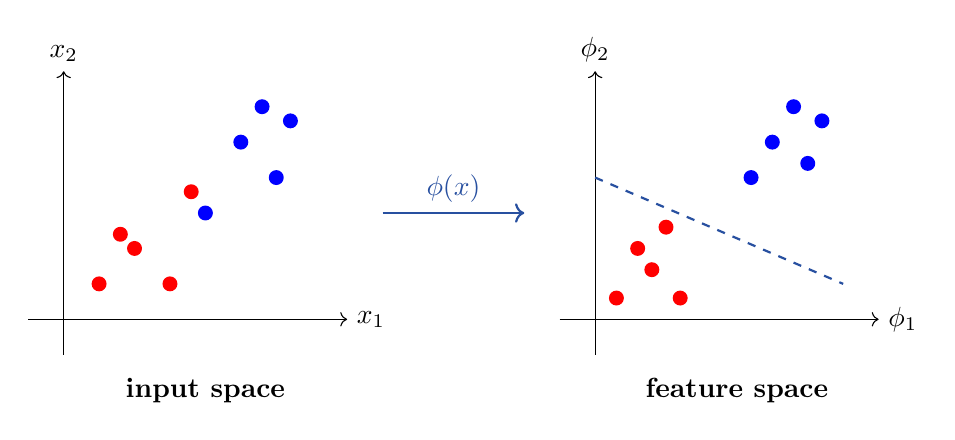
\begin{tikzpicture}[scale=0.9]
    % original space
    \draw[->] (-0.5, 0) -- (4, 0) node[right] {$x_1$};
    \draw[->] (0, -0.5) -- (0, 3.5) node[above] {$x_2$};
    \node at (2, -1) {\textbf{input space}};

    % data points - not separable
    \foreach \x/\y in {0.5/0.5, 1/1, 1.5/0.5, 0.8/1.2} {
        \fill[red] (\x, \y) circle (3pt);
    }
    \foreach \x/\y in {2.5/2.5, 3/2, 2.8/3, 3.2/2.8} {
        \fill[blue] (\x, \y) circle (3pt);
    }
    % overlap region
    \fill[red] (1.8, 1.8) circle (3pt);
    \fill[blue] (2, 1.5) circle (3pt);

    % arrow
    \draw[->, thick, circuitblue] (4.5, 1.5) -- (6.5, 1.5) node[midway, above] {$\phi(x)$};

    % feature space
    \begin{scope}[shift={(7.5, 0)}]
        \draw[->] (-0.5, 0) -- (4, 0) node[right] {$\phi_1$};
        \draw[->] (0, -0.5) -- (0, 3.5) node[above] {$\phi_2$};
        \node at (2, -1) {\textbf{feature space}};

        % now separable
        \foreach \x/\y in {0.3/0.3, 0.8/0.7, 1.2/0.3, 0.6/1, 1/1.3} {
            \fill[red] (\x, \y) circle (3pt);
        }
        \foreach \x/\y in {2.5/2.5, 3/2.2, 2.8/3, 3.2/2.8, 2.2/2} {
            \fill[blue] (\x, \y) circle (3pt);
        }

        % separating hyperplane
        \draw[thick, dashed, circuitblue] (0, 2) -- (3.5, 0.5);
    \end{scope}
\end{tikzpicture}
\end{center}

the whole point of feature maps: make data linearly separable in a higher-dimensional space. quantum circuits do this naturally bcs the hilbert space is exponentially large.

%% ========================================================
\section{Variational Quantum Classifier (VQC)}
%% ========================================================

\subsection{The Big Picture}

a VQC has three stages:

\begin{center}
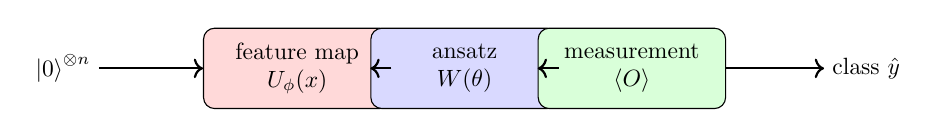
\begin{tikzpicture}[node distance=2.5cm, scale=0.85, every node/.style={scale=0.85}]
    \node[draw, rounded corners, fill=red!15, minimum width=2.8cm, minimum height=1.2cm, align=center] (enc) {feature map\\$U_\phi(x)$};
    \node[draw, rounded corners, fill=blue!15, minimum width=2.8cm, minimum height=1.2cm, right of=enc, align=center] (ans) {ansatz\\$W(\theta)$};
    \node[draw, rounded corners, fill=green!15, minimum width=2.8cm, minimum height=1.2cm, right of=ans, align=center] (meas) {measurement\\$\langle O \rangle$};

    \node[left of=enc, xshift=-1cm] (input) {$\ket{0}^{\otimes n}$};
    \node[right of=meas, xshift=1cm] (output) {class $\hat{y}$};

    \draw[->, thick] (input) -- (enc);
    \draw[->, thick] (enc) -- (ans);
    \draw[->, thick] (ans) -- (meas);
    \draw[->, thick] (meas) -- (output);
\end{tikzpicture}
\end{center}

\begin{enumerate}
    \item \textbf{feature map} $U_\phi(x)$: encodes classical data $x$ into a quantum state
    \item \textbf{ansatz} $W(\theta)$: trainable parameterized circuit
    \item \textbf{measurement}: extract a classical prediction from the quantum state
\end{enumerate}

the full unitary is $U(x, \theta) = W(\theta) U_\phi(x)$, and the output is:
\[
f(x; \theta) = \bra{0}^{\otimes n} U_\phi^\dagger(x) W^\dagger(\theta) \, O \, W(\theta) U_\phi(x) \ket{0}^{\otimes n}
\]

where $O$ is the measurement observable (e.g., $Z_0$ on the first qubit).

\subsection{Stage 1: Feature Map (Encoding)}

the feature map encodes classical data into a quantum state. weve seen these in lecture 09, but lets be specific about the ones used in VQCs.

\textbf{ZFeatureMap:}
\[
U_\phi(x) = \prod_{\ell=1}^{r} \left[\bigotimes_{i=1}^n R_Z(x_i) \cdot H^{\otimes n}\right]
\]

for 1 repetition ($r = 1$), on 3 qubits:
\begin{center}
\begin{quantikz}
\lstick{$\ket{0}$} & \gate{H} & \gate{R_Z(x_1)} & \qw \\
\lstick{$\ket{0}$} & \gate{H} & \gate{R_Z(x_2)} & \qw \\
\lstick{$\ket{0}$} & \gate{H} & \gate{R_Z(x_3)} & \qw
\end{quantikz}
\end{center}

this creates the state:
\[
\ket{\phi(x)} = \bigotimes_{i=1}^n \frac{1}{\sqrt{2}}\left(\ket{0} + e^{ix_i}\ket{1}\right)
\]

each qubit encodes one feature as a phase. no entanglement $\Rightarrow$ tensor product structure.

\textbf{ZZFeatureMap:}
\[
U_\phi(x) = \prod_{\ell=1}^{r}\left[\prod_{i<j} e^{i(\pi - x_i)(\pi - x_j)Z_i Z_j} \cdot \prod_{i} R_Z(2x_i) \cdot H^{\otimes n}\right]
\]

for 2 qubits, 1 rep:
\begin{center}
\begin{quantikz}
\lstick{$\ket{0}$} & \gate{H} & \gate{R_Z(2x_1)} & \ctrl{1} & \gate{R_Z(2(\pi-x_1)(\pi-x_2))} & \ctrl{1} & \qw \\
\lstick{$\ket{0}$} & \gate{H} & \gate{R_Z(2x_2)} & \targ{} & \qw & \targ{} & \qw
\end{quantikz}
\end{center}

the $ZZ$ interaction creates entanglement between qubits, encoding pairwise feature correlations. this is the encoding from havl\'i\v{c}ek et al. (2019) --- the one that led to the quantum kernel method.

\begin{keypoint}
the choice of feature map determines the quantum feature space. ZFeatureMap gives a tensor product (unentangled) feature space. ZZFeatureMap gives an entangled feature space that can encode feature interactions. the entangled version is much harder to simulate classically.
\end{keypoint}

\textbf{PauliFeatureMap (general):}
\[
U_\phi(x) = \prod_{\ell=1}^{r}\left[\exp\left(i\sum_{S \subseteq [n]} \phi_S(x) \prod_{j \in S} P_j\right) \cdot H^{\otimes n}\right]
\]
where $P_j \in \{I, X, Y, Z\}$ and $\phi_S(x) = \prod_{j \in S} x_j$ encodes feature products. ZFeatureMap is the special case with $|S| = 1$ and $P = Z$. ZZFeatureMap adds $|S| = 2$ terms.

\subsection{Stage 2: Ansatz (Trainable Circuit)}

the ansatz is the parameterized part we optimize. two main choices in qiskit:

\textbf{RealAmplitudes ansatz:}
\[
W(\theta) = \prod_{\ell=1}^{L}\left[\text{CNOT layer} \cdot \bigotimes_{i=1}^n R_Y(\theta_i^{(\ell)})\right]
\]

for 3 qubits, 2 layers:
\begin{center}
\begin{quantikz}
\lstick{} & \gate{R_Y(\theta_1^{(1)})} & \ctrl{1} & \qw & \gate{R_Y(\theta_1^{(2)})} & \ctrl{1} & \qw & \gate{R_Y(\theta_1^{(3)})} & \qw \\
\lstick{} & \gate{R_Y(\theta_2^{(1)})} & \targ{} & \ctrl{1} & \gate{R_Y(\theta_2^{(2)})} & \targ{} & \ctrl{1} & \gate{R_Y(\theta_2^{(3)})} & \qw \\
\lstick{} & \gate{R_Y(\theta_3^{(1)})} & \qw & \targ{} & \gate{R_Y(\theta_3^{(2)})} & \qw & \targ{} & \gate{R_Y(\theta_3^{(3)})} & \qw
\end{quantikz}
\end{center}

called ``RealAmplitudes'' bcs $R_Y$ rotations only produce real amplitudes (no complex phases). this is the go-to ansatz for many VQC implementations.

parameter count: $n \times (L + 1)$ for $n$ qubits and $L$ entangling layers.

\textbf{EfficientSU2 ansatz:}
\[
W(\theta) = \prod_{\ell=1}^{L}\left[\text{CNOT layer} \cdot \bigotimes_{i=1}^n R_Y(\theta_{i,1}^{(\ell)}) R_Z(\theta_{i,2}^{(\ell)})\right]
\]

adds $R_Z$ rotations for complex amplitudes. more expressive but more parameters: $2n \times (L+1)$.

\subsection{Stage 3: Measurement}

we need to extract a classical prediction from the quantum state. two approaches:

\textbf{approach 1: estimator primitive (expectation value)}

measure the expectation value of an observable:
\[
\hat{y}(x) = \bra{\psi(x,\theta)} O \ket{\psi(x,\theta)}
\]

common choice: $O = Z_0$ (pauli $Z$ on first qubit), giving $\hat{y} \in [-1, 1]$.

for binary classification: predict class 0 if $\hat{y} > 0$, class 1 if $\hat{y} \leq 0$.

for probabilistic output: map to $[0, 1]$ via $P(y=1) = \frac{1 - \hat{y}}{2}$.

\textbf{approach 2: sampler primitive (probabilities)}

measure all qubits in computational basis. classify based on measurement outcome probabilities:
\[
P(y = k) = \sum_{z : \text{parity}(z) = k} |\braket{z|\psi(x,\theta)}|^2
\]

or more simply: predict class 0 if the first qubit measures $\ket{0}$ more often than $\ket{1}$.

\begin{keypoint}
the estimator primitive gives $\langle O \rangle$ directly (efficient, one number). the sampler primitive gives the full probability distribution (more info, but u need to process it). for binary classification, the estimator with $O = Z_0$ is usually sufficient.
\end{keypoint}

\subsection{The Full VQC Circuit}

putting it all together --- ZZFeatureMap (2 qubits, 1 rep) + RealAmplitudes (1 layer):

\begin{center}
\begin{quantikz}
\lstick{$\ket{0}$} & \gate{H} & \gate{R_Z(2x_1)} & \ctrl{1} & \gate{R_Z(\phi_{12})} & \ctrl{1} & \gate{R_Y(\theta_1)} & \ctrl{1} & \gate{R_Y(\theta_3)} & \meter{} \\
\lstick{$\ket{0}$} & \gate{H} & \gate{R_Z(2x_2)} & \targ{} & \qw & \targ{} & \gate{R_Y(\theta_2)} & \targ{} & \gate{R_Y(\theta_4)} & \qw
\end{quantikz}
\end{center}

where $\phi_{12} = 2(\pi - x_1)(\pi - x_2)$. total: 4 trainable parameters ($\theta_1, \ldots, \theta_4$), 2 data-dependent parameters ($x_1, x_2$).

%% ========================================================
\section{How VQC Works as a Classifier}
%% ========================================================

\subsection{The Classification Pipeline}

\begin{center}
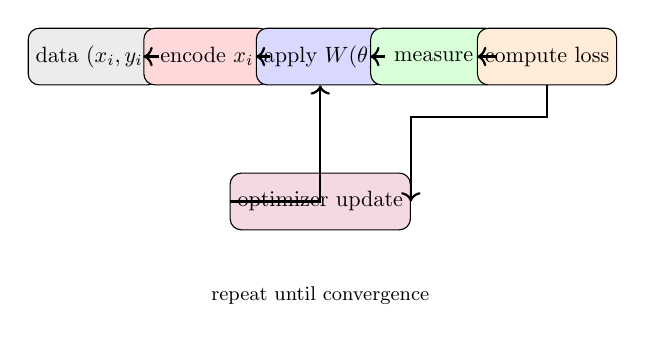
\begin{tikzpicture}[node distance=1.8cm, scale=0.8, every node/.style={scale=0.8}]
    \node[draw, rounded corners, fill=gray!15, minimum width=2cm, minimum height=0.9cm] (data) {data $(x_i, y_i)$};
    \node[draw, rounded corners, fill=red!15, minimum width=2cm, minimum height=0.9cm, right of=data] (encode) {encode $x_i$};
    \node[draw, rounded corners, fill=blue!15, minimum width=2cm, minimum height=0.9cm, right of=encode] (ansatz) {apply $W(\theta)$};
    \node[draw, rounded corners, fill=green!15, minimum width=2cm, minimum height=0.9cm, right of=ansatz] (measure) {measure};
    \node[draw, rounded corners, fill=orange!15, minimum width=2cm, minimum height=0.9cm, right of=measure] (loss) {compute loss};
    \node[draw, rounded corners, fill=purple!15, minimum width=2.2cm, minimum height=0.9cm, below of=ansatz, yshift=-0.5cm] (opt) {optimizer update};

    \draw[->, thick] (data) -- (encode);
    \draw[->, thick] (encode) -- (ansatz);
    \draw[->, thick] (ansatz) -- (measure);
    \draw[->, thick] (measure) -- (loss);
    \draw[->, thick] (loss.south) -- ++(0, -0.5) -| (opt.east);
    \draw[->, thick] (opt.west) -| (ansatz.south);
    \node[below of=opt, yshift=0.3cm] {\small repeat until convergence};
\end{tikzpicture}
\end{center}

step by step:
\begin{enumerate}
    \item take a training sample $(x_i, y_i)$
    \item encode $x_i$ into the quantum state via $U_\phi(x_i)\ket{0}^{\otimes n}$
    \item apply the trainable ansatz $W(\theta)$
    \item measure to get prediction $\hat{y}_i$
    \item compute the loss $\mathcal{L}(\hat{y}_i, y_i)$
    \item use a classical optimizer to update $\theta$
    \item repeat over the training set until convergence
\end{enumerate}

\subsection{Forward Pass in Detail}

for input $x$:
\begin{align}
\ket{\psi_0} &= \ket{0}^{\otimes n} \quad \text{(initial state)} \\
\ket{\psi_1} &= U_\phi(x)\ket{\psi_0} \quad \text{(encoded state)} \\
\ket{\psi_2} &= W(\theta)\ket{\psi_1} \quad \text{(after ansatz)} \\
\hat{y} &= \bra{\psi_2} O \ket{\psi_2} \quad \text{(measurement)}
\end{align}

expanding:
\[
\hat{y}(x;\theta) = \bra{0}^{\otimes n} U_\phi^\dagger(x) W^\dagger(\theta) \, O \, W(\theta) U_\phi(x) \ket{0}^{\otimes n}
\]

this is a function $f: \mathbb{R}^d \times \mathbb{R}^p \to [-1, 1]$ where $d$ = data dimension, $p$ = number of parameters.

\subsection{Encoding Data: What Happens Geometrically}

when we encode $x$ via $U_\phi(x)\ket{0}^{\otimes n}$, we map $x$ to a point on the unit sphere in $\mathbb{C}^{2^n}$ (or equivalently, a point on the bloch hypersphere for $n > 1$).

\begin{example}
for 1 qubit with $U_\phi(x) = R_Y(x)$:
\[
\ket{\phi(x)} = \cos\frac{x}{2}\ket{0} + \sin\frac{x}{2}\ket{1}
\]
this traces out a great circle on the bloch sphere as $x$ varies. the encoding maps the 1D input to a curve on a 2D sphere.

for 2 qubits with tensor product encoding:
\[
\ket{\phi(x_1, x_2)} = R_Y(x_1)\ket{0} \otimes R_Y(x_2)\ket{0}
\]
the feature space is $\mathbb{C}^4$ (a 4-dimensional state). we go from 2D classical to effectively 4D quantum.
\end{example}

\subsection{The Ansatz: Learning a Rotation}

the ansatz $W(\theta)$ is a parameterized unitary. geometrically, it rotates the encoded state in hilbert space. training $\theta$ = finding the rotation that aligns same-class states in one direction and different-class states in another.

\begin{intuition}
think of it this way: the feature map puts data points on a sphere. the ansatz rotates the sphere so that a fixed measurement axis (say, $Z$) separates the classes. the optimizer finds the rotation angles $\theta$ that achieve the best separation.
\end{intuition}

\subsection{Parameterized Layers and Expressibility}

more layers in the ansatz = more expressive model:
\begin{itemize}
    \item 0 layers (identity ansatz): the classifier is completely determined by the feature map + measurement. no learnable parameters.
    \item 1 layer: can learn simple rotations. equivalent to a linear model in feature space (well prove this later).
    \item $L$ layers: increasing expressibility. the circuit can represent more complex decision boundaries.
    \item $\sim n$ layers: the circuit becomes approximately universal --- can represent any unitary.
\end{itemize}

but theres a catch: more layers $\Rightarrow$ more parameters $\Rightarrow$ harder optimization (barren plateaus, lecture 16).

%% ========================================================
\section{Cost Functions for Classification}
%% ========================================================

\subsection{Parity-Based Cost}

the simplest approach: use the expectation value of $Z_0$ directly as a loss:
\[
\mathcal{L}(\theta) = \frac{1}{N}\sum_{i=1}^N (y_i - \hat{y}_i(\theta))^2
\]
where $y_i \in \{-1, +1\}$ and $\hat{y}_i = \braket{Z_0}_{x_i, \theta}$.

this is just MSE loss on the quantum output. simple but works.

\subsection{Cross-Entropy Loss (Adapted)}

for probabilistic classification, map the quantum output to probabilities:
\[
p_i = P(y_i = 1 | x_i, \theta) = \frac{1 - \braket{Z_0}_{x_i, \theta}}{2}
\]

then use binary cross-entropy:
\[
\mathcal{L}(\theta) = -\frac{1}{N}\sum_{i=1}^N\left[\tilde{y}_i \log p_i + (1 - \tilde{y}_i)\log(1 - p_i)\right]
\]
where $\tilde{y}_i \in \{0, 1\}$ (relabeled from $\{-1, +1\}$).

\begin{keypoint}
cross-entropy loss has steeper gradients than MSE when predictions r confident but wrong. this often leads to faster convergence for VQCs. in qiskit, the \texttt{NeuralNetworkClassifier} supports both.
\end{keypoint}

\subsection{Hinge Loss (SVM-style)}

adapted from SVMs:
\[
\mathcal{L}(\theta) = \frac{1}{N}\sum_{i=1}^N \max(0, 1 - y_i \cdot \hat{y}_i(\theta))
\]

penalizes predictions that r on the wrong side of the margin. zero loss when $y_i \cdot \hat{y}_i \geq 1$, i.e., when the prediction is correct with margin.

\subsection{Multi-Class Extension}

for $C > 2$ classes, use $C$ measurement qubits or $C$ observables:
\[
\hat{y}(x) = \arg\max_{c \in \{0, \ldots, C-1\}} \braket{O_c}_{x, \theta}
\]

where $O_c = Z_c$ (measure the $c$-th qubit). combine with softmax cross-entropy:
\[
P(y = c | x) = \frac{e^{\braket{O_c}}}{\sum_{c'} e^{\braket{O_{c'}}}}
\]

%% ========================================================
\section{The Classical Optimization Loop}
%% ========================================================

\subsection{How Optimization Works}

the optimizer is entirely classical. it receives the loss value (and possibly gradients) from the quantum circuit and updates parameters.

\begin{center}
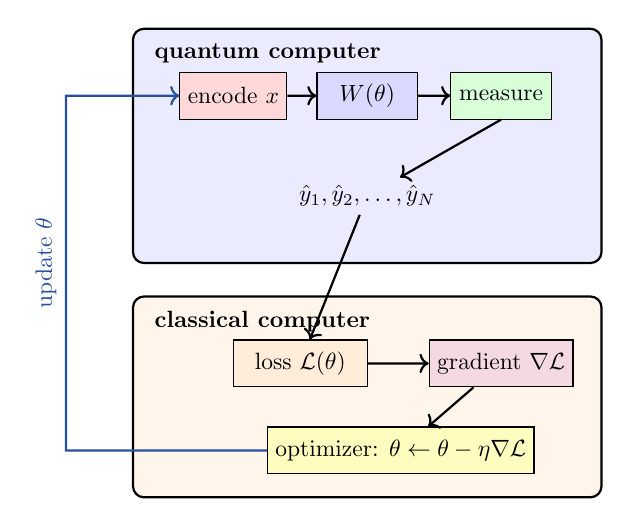
\begin{tikzpicture}[scale=0.85, every node/.style={scale=0.85}]
    % quantum computer box
    \draw[thick, rounded corners, fill=blue!8] (-0.5, 0) rectangle (6.5, 3.5);
    \node[anchor=north west] at (-0.3, 3.4) {\textbf{quantum computer}};

    \node[draw, fill=red!15, minimum width=1.5cm, minimum height=0.7cm] at (1, 2.5) (enc) {encode $x$};
    \node[draw, fill=blue!15, minimum width=1.5cm, minimum height=0.7cm] at (3, 2.5) (ans) {$W(\theta)$};
    \node[draw, fill=green!15, minimum width=1.5cm, minimum height=0.7cm] at (5, 2.5) (meas) {measure};

    \draw[->, thick] (enc) -- (ans);
    \draw[->, thick] (ans) -- (meas);

    \node at (3, 1) (val) {$\hat{y}_1, \hat{y}_2, \ldots, \hat{y}_N$};
    \draw[->, thick] (meas.south) -- (val);

    % classical computer box
    \draw[thick, rounded corners, fill=orange!8] (-0.5, -3.5) rectangle (6.5, -0.5);
    \node[anchor=north west] at (-0.3, -0.6) {\textbf{classical computer}};

    \node[draw, fill=orange!15, minimum width=2cm, minimum height=0.7cm] at (2, -1.5) (loss) {loss $\mathcal{L}(\theta)$};
    \node[draw, fill=purple!15, minimum width=2cm, minimum height=0.7cm] at (5, -1.5) (grad) {gradient $\nabla\mathcal{L}$};
    \node[draw, fill=yellow!25, minimum width=2.5cm, minimum height=0.7cm] at (3.5, -2.8) (opt) {optimizer: $\theta \leftarrow \theta - \eta\nabla\mathcal{L}$};

    \draw[->, thick] (val) -- (loss);
    \draw[->, thick] (loss) -- (grad);
    \draw[->, thick] (grad) -- (opt);

    % feedback loop
    \draw[->, thick, circuitblue] (opt.west) -| (-1.5, 2.5) -- (enc.west);
    \node[circuitblue, rotate=90] at (-1.8, 0) {update $\theta$};
\end{tikzpicture}
\end{center}

\subsection{Gradient Computation}

two main approaches:

\textbf{parameter shift rule:}
\[
\frac{\partial \mathcal{L}}{\partial \theta_k} = \frac{\mathcal{L}(\theta_k + \pi/2) - \mathcal{L}(\theta_k - \pi/2)}{2}
\]

requires 2 circuit evaluations per parameter. for $p$ parameters: $2p$ circuits per gradient step.

\textbf{finite difference:}
\[
\frac{\partial \mathcal{L}}{\partial \theta_k} \approx \frac{\mathcal{L}(\theta_k + \epsilon) - \mathcal{L}(\theta_k - \epsilon)}{2\epsilon}
\]

less accurate (approximation), but same cost. the parameter shift rule is exact for gates of the form $e^{-i\theta G/2}$ where $G^2 = I$.

\textbf{gradient-free optimizers:}
COBYLA, Nelder-Mead, SPSA. dont need gradients at all. SPSA is particularly useful bcs it estimates the gradient with only 2 circuit evaluations (regardless of $p$):
\[
\hat{g}_k = \frac{\mathcal{L}(\theta + c\Delta) - \mathcal{L}(\theta - c\Delta)}{2c\Delta_k}
\]
where $\Delta$ is a random perturbation vector.

\subsection{Common Optimizers for VQC}

\begin{center}
\begin{tabular}{l|c|c|l}
\textbf{optimizer} & \textbf{gradient?} & \textbf{circuits/step} & \textbf{notes} \\
\hline
COBYLA & no & 1--few & simple, often good enough \\
SPSA & stochastic & 2 & great for noisy hardware \\
Adam & yes & $2p + 1$ & fast convergence, needs gradients \\
L-BFGS-B & yes & $2p + 1$ & good for simulators \\
NFT & no & $O(p)$ & designed for quantum circuits
\end{tabular}
\end{center}

\begin{keypoint}
on real hardware, use SPSA or COBYLA --- they handle shot noise well. on simulators, use Adam or L-BFGS-B for faster convergence. the parameter shift rule is mathematically exact but expensive ($2p$ circuits per step).
\end{keypoint}

%% ========================================================
\section{From Variational to Linear: The Key Insight}
%% ========================================================

\subsection{The Surprising Connection}

heres the deep result. consider a VQC with:
\begin{itemize}
    \item feature map $U_\phi(x)$
    \item ansatz $W(\theta)$
    \item observable $O$
\end{itemize}

the output is:
\[
f(x; \theta) = \bra{0} U_\phi^\dagger(x) W^\dagger(\theta) \, O \, W(\theta) U_\phi(x) \ket{0}
\]

define the ``rotated observable'':
\[
\tilde{O}(\theta) = W^\dagger(\theta) \, O \, W(\theta)
\]

this is a fixed hermitian operator (for given $\theta$). now:
\[
f(x; \theta) = \bra{0} U_\phi^\dagger(x) \, \tilde{O}(\theta) \, U_\phi(x) \ket{0} = \text{Tr}\left[\tilde{O}(\theta) \cdot \rho(x)\right]
\]

where $\rho(x) = U_\phi(x)\ket{0}\bra{0}U_\phi^\dagger(x)$ is the encoded density matrix.

\begin{keypoint}
the VQC output is a \textbf{linear function} of the density matrix $\rho(x)$! the density matrix is the feature vector, and $\tilde{O}(\theta)$ plays the role of the weight matrix. the ansatz parameters $\theta$ only determine the weight matrix --- they dont change the features.
\end{keypoint}

\subsection{Making It Explicit}

expand $\tilde{O}(\theta)$ in the pauli basis:
\[
\tilde{O}(\theta) = \sum_{\alpha} w_\alpha(\theta) \, P_\alpha
\]
where $P_\alpha \in \{I, X, Y, Z\}^{\otimes n}$ are the $4^n$ pauli strings and $w_\alpha(\theta)$ are real coefficients determined by $\theta$.

then:
\[
f(x; \theta) = \sum_\alpha w_\alpha(\theta) \cdot \text{Tr}[P_\alpha \rho(x)] = \sum_\alpha w_\alpha(\theta) \cdot \phi_\alpha(x)
\]

where $\phi_\alpha(x) = \text{Tr}[P_\alpha \rho(x)]$ are the quantum features (expectation values of pauli operators on the encoded state).

this is literally a \textbf{linear model}:
\[
f(x; \theta) = w(\theta)^\top \phi(x)
\]

with feature vector $\phi(x) \in \mathbb{R}^{4^n}$ and weight vector $w(\theta) \in \mathbb{R}^{4^n}$.

\subsection{The Implications}

\begin{enumerate}
    \item the VQC is a linear classifier in the quantum feature space, regardless of circuit depth
    \item nonlinearity comes from the feature map $\phi(x) = \text{Tr}[P_\alpha \rho(x)]$, not from the ansatz
    \item the ansatz only determines which linear combination of features to use
    \item this is exactly analogous to classical kernel methods: nonlinear in input space, linear in feature space
\end{enumerate}

\begin{intuition}
the feature map does all the heavy lifting. the ansatz is just choosing a direction in feature space. making the ansatz more complex (deeper, more parameters) gives u more ``directions'' to choose from, but the classifier is still fundamentally linear in the quantum features.
\end{intuition}

\subsection{Proof Sketch}

\textbf{claim:} for any VQC with feature map $U_\phi$, ansatz $W(\theta)$, and observable $O$, the model output $f(x;\theta) = \text{Tr}[\tilde{O}(\theta) \rho(x)]$ is linear in the density matrix features.

\textbf{proof:}
\begin{enumerate}
    \item the trace is a linear operation: $\text{Tr}[A(\alpha B + \beta C)] = \alpha\text{Tr}[AB] + \beta\text{Tr}[AC]$
    \item $\tilde{O}(\theta)$ is a fixed operator for given $\theta$
    \item therefore $f(x;\theta) = \text{Tr}[\tilde{O}(\theta)\rho(x)]$ is linear in $\rho(x)$
    \item since $\rho(x) = \ket{\phi(x)}\bra{\phi(x)}$, the features $\phi_\alpha(x) = \text{Tr}[P_\alpha \rho(x)]$ span the feature space
    \item so $f$ is a linear function of the features $\phi_\alpha$ \qed
\end{enumerate}

\subsection{Connection to Kernel Methods}

this directly connects VQCs to quantum kernels:

the quantum kernel is:
\[
\kappa(x, x') = \text{Tr}[\rho(x)\rho(x')] = |\braket{\phi(x)|\phi(x')}|^2
\]

since the VQC is linear in $\rho(x)$, and the kernel is the inner product $\text{Tr}[\rho(x)\rho(x')]$ in the density matrix space, the VQC is doing exactly what a kernel SVM does: linear classification in a high-dimensional feature space, with the kernel encoding the inner products.

\begin{keypoint}
\textbf{the punchline:} VQC $\equiv$ kernel method. training a VQC is equivalent to finding a linear classifier in the quantum kernel feature space. this means all the theory of kernel methods (generalization bounds, representer theorem, etc.) applies directly to VQCs.
\end{keypoint}

%% ========================================================
\section{When Does the Variational Approach Help?}
%% ========================================================

\subsection{VQC vs Direct Kernel Method}

if VQCs r just kernel methods in disguise, why not use the kernel directly?

\textbf{advantages of VQC (variational) approach:}
\begin{itemize}
    \item scales better with dataset size: $O(N)$ circuit evaluations per epoch vs $O(N^2)$ for the kernel matrix
    \item natural for online learning (can update with one sample at a time)
    \item can learn feature-dependent weights (if using data re-uploading)
    \item easier to implement on near-term hardware (one circuit per sample)
\end{itemize}

\textbf{advantages of kernel approach:}
\begin{itemize}
    \item convex optimization (no local minima)
    \item well-understood generalization theory
    \item no barren plateaus (the kernel is computed, not optimized)
    \item provably finds the optimal linear classifier in feature space
\end{itemize}

\subsection{When VQC Goes Beyond Kernel}

the linear equivalence holds when the ansatz is applied AFTER the encoding. but there r ways to break it:

\textbf{data re-uploading (P\'erez-Salinas et al. 2020):}
\[
U(x, \theta) = \prod_\ell W(\theta_\ell) U_\phi(x)
\]
interleave encoding and trainable layers. this creates a nonlinear dependence on $x$ in the effective observable, going beyond the kernel framework.

\textbf{adaptive encoding:}
\[
U_\phi(x, \theta_{\text{enc}}) = \text{encoding that depends on trainable parameters}
\]
the feature map itself is learned. this is like learning the kernel, which goes beyond fixed-kernel methods.

%% ========================================================
\section{Limitations of the Variational Approach}
%% ========================================================

\subsection{Local Minima}

the VQC loss landscape is generally non-convex. gradient descent can get stuck in local minima that r far from the global optimum.

\begin{example}
for a 4-qubit VQC with 20 parameters, the loss landscape has many local minima regions. random initialization means u start in a random one and may never find the global minimum. in contrast, the kernel SVM finds the global optimum (convex problem).
\end{example}

\subsection{Shot Noise}

on real hardware, expectation values r estimated from finite measurements:
\[
\braket{Z_0} \approx \frac{1}{S}\sum_{s=1}^S z_0^{(s)} \quad \text{where } z_0^{(s)} \in \{-1, +1\}
\]

the variance is:
\[
\text{Var}[\hat{y}] = \frac{1 - \braket{Z_0}^2}{S}
\]

for $S = 1000$ shots: standard deviation $\sim 0.03$. this noise propagates to gradients:
\[
\text{Var}\left[\frac{\partial \hat{y}}{\partial \theta_k}\right] \sim \frac{1}{S}
\]

noisy gradients slow convergence and can cause oscillations near the optimum.

\subsection{Circuit Depth}

deeper circuits $=$ more noise on real hardware. for current devices with 2-qubit gate error $p \sim 10^{-3}$ to $10^{-2}$:
\[
\text{circuit fidelity} \approx (1-p)^{N_{\text{2Q gates}}}
\]

a VQC with 10 qubits, 3 ansatz layers, and ZZFeatureMap might need $\sim 100$ two-qubit gates. at $p = 5 \times 10^{-3}$:
\[
F \approx (0.995)^{100} \approx 0.61
\]

thats 39\% noise floor. the classifier is fighting a losing battle.

\subsection{Barren Plateaus (Preview)}

as well see in lecture 16, random deep circuits have exponentially vanishing gradients:
\[
\text{Var}\left[\frac{\partial \mathcal{L}}{\partial \theta_k}\right] \leq O(2^{-n})
\]

for 20 qubits: gradient variance $\sim 10^{-6}$. u need $\sim 10^{12}$ shots to detect these gradients above shot noise. completely impractical.

\begin{keypoint}
the three horsemen of VQC doom: local minima, shot noise, and barren plateaus. all three get worse as u scale up. this is why the kernel perspective is so valuable --- it lets u analyze VQCs without actually doing the optimization.
\end{keypoint}

%% ========================================================
\section{Practical Considerations}
%% ========================================================

\subsection{Choosing the Feature Map}

\begin{center}
\begin{tabular}{l|c|c|l}
\textbf{feature map} & \textbf{entanglement} & \textbf{depth} & \textbf{when to use} \\
\hline
ZFeatureMap & none & $O(1)$ & simple datasets, fast \\
ZZFeatureMap & pairwise & $O(n^2)$ & feature interactions matter \\
PauliFeatureMap & custom & varies & u know the problem structure \\
angle encoding & none & $O(1)$ & baseline, always try first
\end{tabular}
\end{center}

\subsection{Choosing the Ansatz}

\begin{center}
\begin{tabular}{l|c|c|l}
\textbf{ansatz} & \textbf{params} & \textbf{entangling gates} & \textbf{when to use} \\
\hline
RealAmplitudes & $n(L+1)$ & $L(n-1)$ & default choice \\
EfficientSU2 & $2n(L+1)$ & $L(n-1)$ & need more expressibility \\
TwoLocal & custom & custom & hardware-specific design
\end{tabular}
\end{center}

\subsection{Choosing the Optimizer}

rule of thumb:
\begin{itemize}
    \item \textbf{simulator}: L-BFGS-B or Adam (exact gradients, fast convergence)
    \item \textbf{real hardware}: SPSA (handles shot noise, 2 circuits per step) or COBYLA (gradient-free)
    \item \textbf{large parameter count}: SPSA (gradient cost independent of $p$)
\end{itemize}

\subsection{Hyperparameter Guidelines}

\begin{itemize}
    \item number of qubits $n$: set to input dimension $d$ (or use PCA to reduce $d$ to $n$)
    \item ansatz depth $L$: start with 1--2 layers, increase only if underfitting
    \item feature map reps $r$: 1--2 is usually enough
    \item shots per evaluation: 1024 for prototyping, 4096--8192 for final results
    \item learning rate: $10^{-2}$ to $10^{-1}$ for SPSA, $10^{-3}$ for Adam
    \item max iterations: 100--500 (monitor loss, stop early if converged)
\end{itemize}

%% ========================================================
\section{Example: VQC on Iris Dataset}
%% ========================================================

\subsection{Setup}

the iris dataset: 150 samples, 4 features, 3 classes. well do binary classification on the first 2 classes (setosa vs versicolor, 100 samples).

\textbf{preprocessing:}
\begin{enumerate}
    \item take first 2 classes (100 samples)
    \item standardize features to zero mean, unit variance
    \item scale to $[0, \pi]$ for angle encoding
    \item 80/20 train/test split
\end{enumerate}

\textbf{VQC configuration:}
\begin{itemize}
    \item 4 qubits (one per feature)
    \item ZZFeatureMap, 1 rep
    \item RealAmplitudes ansatz, 2 layers
    \item $O = Z_0$ measurement
    \item COBYLA optimizer, 200 iterations
    \item 1024 shots (simulated)
\end{itemize}

\subsection{Expected Results}

typical performance on iris (2-class):
\begin{itemize}
    \item train accuracy: 95--100\%
    \item test accuracy: 90--100\%
    \item convergence: $\sim 50$--100 iterations
    \item total circuit evaluations: $\sim 100 \times 100 = 10{,}000$ (iterations $\times$ training samples)
\end{itemize}

for comparison, a classical SVM with RBF kernel gets 100\% on this same task. the point isnt to beat classical here --- iris is tiny. the point is to verify the pipeline works.

\subsection{The Qiskit Code Flow}

the qiskit implementation flow (describing, not showing code):
\begin{enumerate}
    \item create the feature map: \texttt{ZZFeatureMap(feature\_dimension=4, reps=1)}
    \item create the ansatz: \texttt{RealAmplitudes(num\_qubits=4, reps=2)}
    \item combine into full circuit: feature map + ansatz
    \item create the classifier: \texttt{VQC(feature\_map, ansatz, optimizer, ...)}
    \item fit: \texttt{vqc.fit(X\_train, y\_train)}
    \item predict: \texttt{vqc.predict(X\_test)}
    \item score: \texttt{vqc.score(X\_test, y\_test)}
\end{enumerate}

%% ========================================================
\section{Summary}
%% ========================================================

key takeaways from this lecture:

\begin{enumerate}
    \item the VQC has three stages: feature map $\to$ ansatz $\to$ measurement
    \item the feature map encodes data into quantum hilbert space; the ansatz provides trainable parameters
    \item the full VQC output is $f(x;\theta) = \text{Tr}[\tilde{O}(\theta)\rho(x)]$ --- a linear function of the density matrix
    \item this means VQCs r linear classifiers in quantum feature space, equivalent to kernel methods
    \item nonlinearity comes from the feature map, not the ansatz
    \item cost functions: MSE, cross-entropy, hinge loss --- all adapted for quantum outputs
    \item optimization loop: quantum circuit evaluation + classical parameter update
    \item parameter shift rule gives exact gradients; SPSA is practical for noisy hardware
    \item limitations: local minima, shot noise, circuit depth, barren plateaus
    \item data re-uploading can break the linear equivalence, going beyond kernel methods
\end{enumerate}

the variational-to-linear connection is one of the most important results in QML theory. it tells us that the feature map is king --- if u want a better VQC, focus on the encoding, not the ansatz.

next lecture: we make the kernel connection explicit and develop quantum feature space theory from the ground up.

\end{document}
